\documentclass{article}
\usepackage[utf8]{inputenc}
\usepackage{geometry}
\usepackage[T1]{fontenc}
\usepackage{amsfonts}
\usepackage{graphicx}
\usepackage{float}
\usepackage{hyperref}
\usepackage[sorting=none]{biblatex}
\usepackage{fancyhdr}
\usepackage{multicol}
\addbibresource{ref.bib}
\setlength{\columnsep}{40pt}
\setlength{\voffset}{0.7cm}
\setlength{\headsep}{40pt}
\geometry{legalpaper, portrait, margin=2cm}


% Title page
\title{Essay title\\\Large{Machine Learning, Advanced Course/DD2434/mladv24}}
\author{Aurhor \\ KTH Royal Institute of Technology\\ School of Engineering Sciences in Chemistry, Biotechnology and Health}
\date{\today}

% Header and footer
\pagestyle{fancy}
\fancyhead{}
\fancyhead[L]{\textbf{Machine Learning, Advanced Course}\\\textbf{DD2434}}
\fancyhead[R]{\textbf{Andrea Stanziale, Leonardo Lüder}\\ stanz@kth.se, luder@kth.se}
\fancyfoot{}
\begin{document}

\maketitle
\thispagestyle{fancy}
\clearpage
\tableofcontents
\thispagestyle{fancy}

\clearpage
% Begin page numbers
\fancyfoot[C]{\thepage}
\pagenumbering{arabic}
\begin{multicols}{2}

    \section*{1.1}

    \section*{1.2}

    \subsection*{1.2.7}
    We implement a function that generates a dataset of $N$ points in the plane, where each point is drawn from a normal distribution with mean $\mu$ and precision $\tau$. For reproducability we set the seed of the random number generator to 0. We generate datasets for $N = 10, 100, 1000$ and plot the generated values as histograms, which results in figure \autoref{fig:histograms_datasets}. 

    
    \begin{figure}[H]
        \centering
        \begin{minipage}{0.32\textwidth}
            \centering
            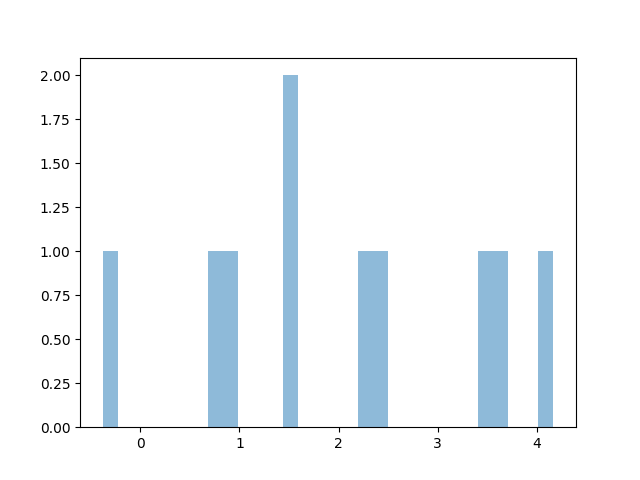
\includegraphics[width=\textwidth]{figures/1.2/dataset_1.png}
            \caption{N=10}
        \end{minipage}
        \hfill
        \begin{minipage}{0.32\textwidth}
            \centering
            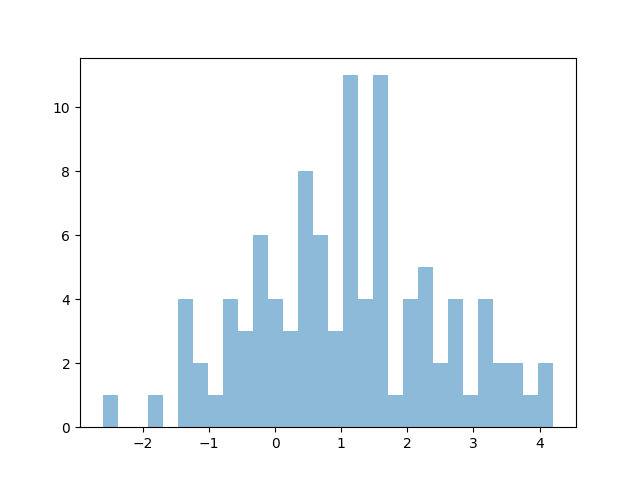
\includegraphics[width=\textwidth]{figures/1.2/dataset_2.png}
            \caption{N=100}
        \end{minipage}
        \hfill
        \begin{minipage}{0.32\textwidth}
            \centering
            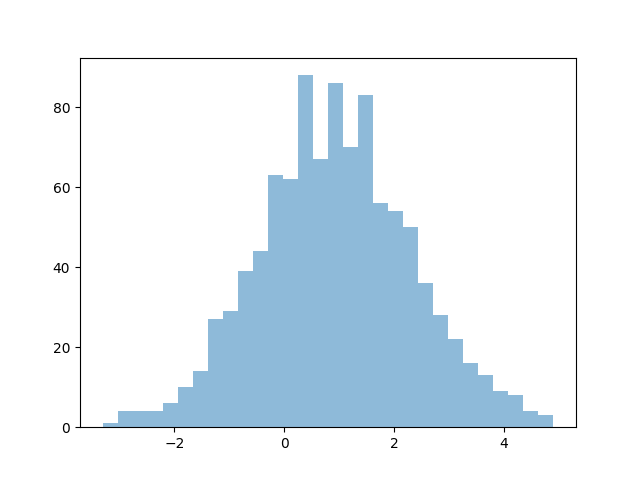
\includegraphics[width=\textwidth]{figures/1.2/dataset_3.png}
            \caption{N=1000}
        \end{minipage}
        \caption{Histograms of generated datasets}\label{fig:histograms_datasets}
    \end{figure}

    We see that the more datapoints we have the more the histogram resembles a normal distribution which is as expected.

    \subsection{1.2.8}

    We derive the ML estimates for $\mu$ and $\tau$. 
    The posterior distribution is proportional to the product of the likelihood and the prior:

\begin{equation}
    p(\mu, \tau | X) \propto p(X | \mu, \tau) p(\mu | \tau) p(\tau)
\end{equation}
    


    The likelihood is given by:

    \begin{equation}
    p(X | \mu, \tau) = \prod_{i=1}^{N} p(X_i | \mu, \tau) = \prod_{i=1}^{N} \sqrt{\frac{\tau}{2 \pi}} e^{-\frac{\tau}{2} (X_i - \mu)^2}
    \end{equation}

    where we assume \( X_i | \mu, \tau \sim N(\mu, \frac{1}{\tau}) \).

    The prior distributions are:

    \begin{equation}
    p(\mu | \tau) = N(\mu_0, \frac{1}{\lambda_0 \tau}); \quad p(\tau) = \mathrm{Gamma}(\alpha_0, \beta_0)
    \end{equation}


    This gives the joint posterior:

    \begin{equation}
    p(\mu, \tau | X) \propto \prod_{i=1}^{N} \sqrt{\frac{\tau}{2 \pi}} e^{-\frac{\tau}{2} (X_i - \mu)^2} \times \sqrt{\frac{\lambda_0 \tau}{2 \pi}} e^{-\frac{\lambda_0 \tau}{2} (\mu - \mu_0)^2} \times \frac{\beta_0^{\alpha_0}}{\Gamma(\alpha_0)} \tau^{\alpha_0 - 1} e^{-\beta_0 \tau}
    \end{equation}

    Simplifying, we get:

    \begin{equation}
    p(\mu, \tau | X) \propto \left(\frac{\tau}{2 \pi}\right)^{\frac{N+1}{2}} e^{-\frac{\tau}{2} \left(\sum_{i=1}^{N} (X_i - \mu)^2 + \lambda_0 (\mu - \mu_0)^2 + 2 \beta_0 \right)} \tau^{\alpha_0 + \frac{N}{2} - 1}
    \end{equation}


    After completing the square for terms involving \( \mu \) and simplifying, the posterior distribution of \( \mu \) given \( X \) and \( \tau \) is:

    \begin{equation}
    p(\mu | X, \tau) \sim N\left(\frac{\sum X_i + \lambda_0 \mu_0}{N + \lambda_0}, \frac{1}{(N + \lambda_0) \tau}\right)
    \end{equation}




\end{multicols}
\clearpage
\addcontentsline{toc}{section}{References}
\printbibliography{}

\end{document}
